\documentclass{beamer}
\usepackage[utf8]{inputenc}

\usetheme{Madrid}
\usecolortheme{default}


\usepackage{natbib}
\bibliographystyle{authoryear}
\bibliography{Reference}

\usepackage{graphicx}
\usepackage{booktabs}
\usepackage{adjustbox}
\usepackage{amsmath, amssymb}
%------------------------------------------------------------
%This block of code defines the information to appear in the
%Title page
\title[Digital Tools For Finance] %optional
{The Impact of News Information Acquisition and Congnition} 

\author[Banking and Finance] % (optional)
{Chuanyi You 22-735-765\and \\
Chuyi Zheng 22-736-425\and \\
Cunyu Zhang 23-718-877\and\\
Zixuan Yang 22-737-795}


\date[December 2023] % (optional)
{Digital Tools for Finance, December 2023}


%End of title page configuration block
%------------------------------------------------------------



%------------------------------------------------------------
%The next block of commands puts the table of contents at the 
%beginning of each section and highlights the current section:

\AtBeginSection[]
{
  \begin{frame}
    \frametitle{Table of Contents}
    \tableofcontents[currentsection]
  \end{frame}
}
%------------------------------------------------------------


\begin{document}

%The next statement creates the title page.
\frame{\titlepage}


%---------------------------------------------------------
%This block of code is for the table of contents after
%the title page
\begin{frame}
\frametitle{Table of Contents}
\tableofcontents
\end{frame}
%---------------------------------------------------------


\section{Background}


\begin{frame}
\frametitle{Background}
\textbf{Information Channels} significantly increased recently and have impact on social attitudes and cognitive behaviors at the individual level.


\vspace{12pt}
\textbf{The ”2019 College Students’ Social Mentality Survey,” }is designed to explore how Chinese college students access news and the subsequent effect on their perception of societal, political, and economic issues.
\end{frame}


%--------------------------------------------------------
\section{Data}

\begin{frame}
\frametitle{Data}
The data set from the ”2019 College Student Information Perception Survey” contains 1,254 entries.
\begin{figure}
  \centering
  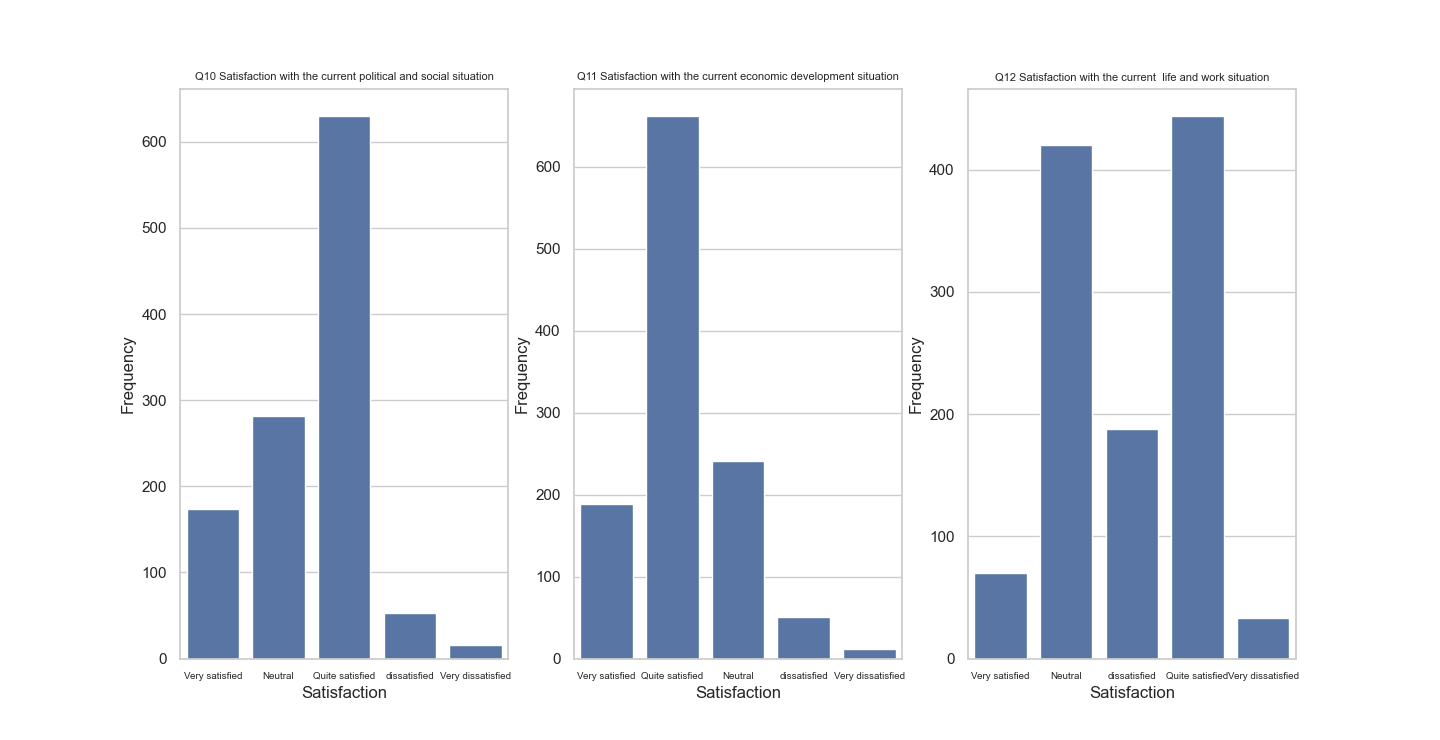
\includegraphics[width=0.8\linewidth]{Distribution.jpg}
  \caption{Descriptive Data of dependent variables}
  \label{fig:Distribution}
\end{figure}
\end{frame}

\begin{frame}
\frametitle{Data}

\begin{figure}
  \centering
  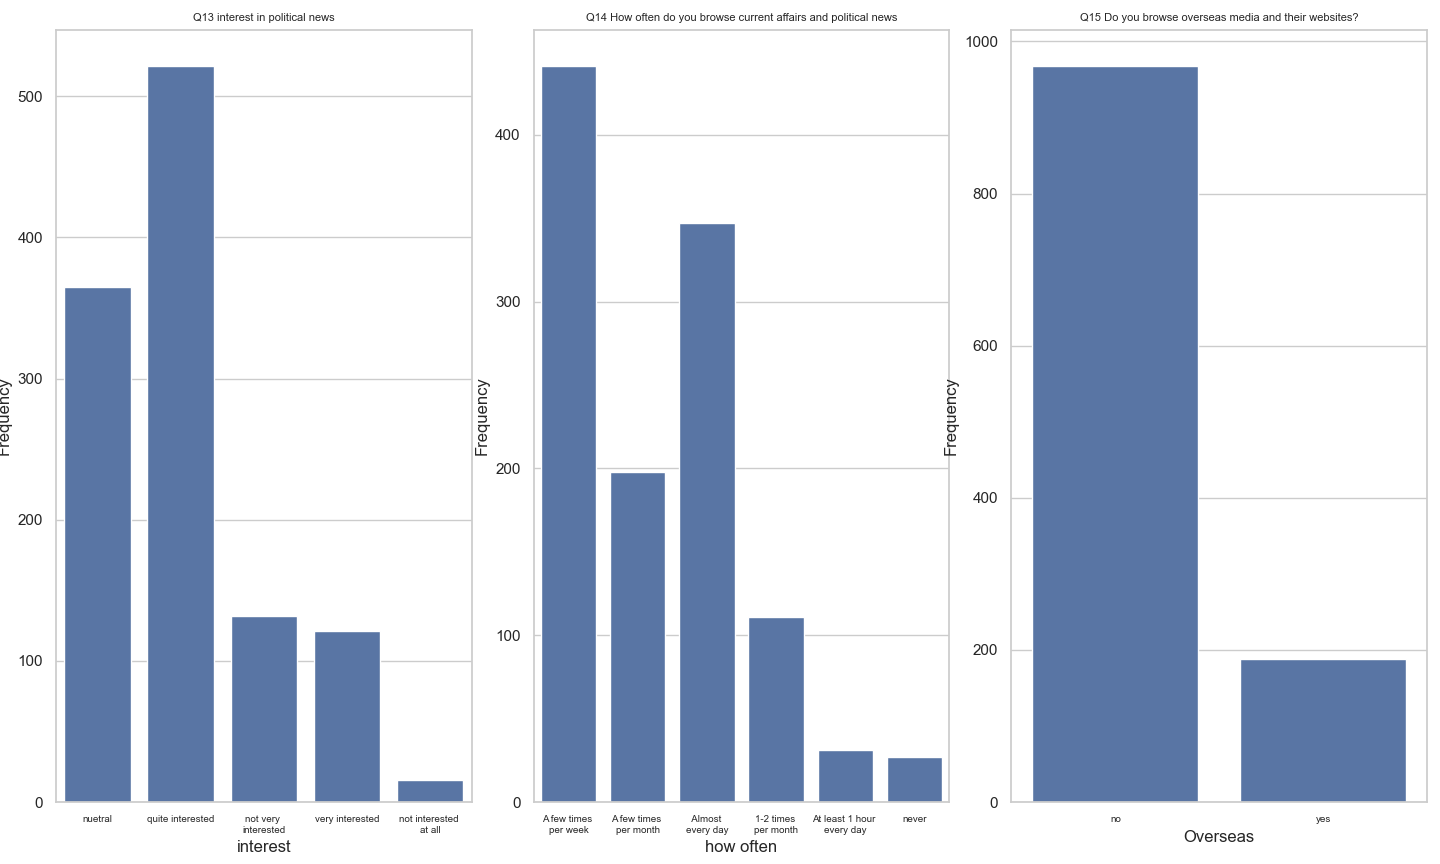
\includegraphics[width=0.8\linewidth]{Distribution2.jpg}
  \caption{Descriptive Data of key independent variables}
  \label{fig:Distribution}
\end{figure}
\end{frame}

%---------------------------------------------------------
\section{Hypothesis}
%Changing visivility of the text
\begin{frame}
\frametitle{Hypothesis}

\begin{itemize}
    \item<1-> \textbf{Hypothesis 1}: College students' \textbf{political and social satisfaction} is significantly influenced by their interest in news, time spent reading news, and obtaining news internationally.
\begin{equation}
\text{pol\_sat} = \beta_0 + \beta_1 \cdot \text{interest} + \beta_2 \cdot \text{time} + \beta_3 \cdot \text{overseas} + \gamma \cdot \text{controls} + \varepsilon_1
\end{equation}

\textit{\small{pol\_ sat: Political and social satisfaction\\
interest: Level of interest in political news\\
time: Frequency of browsing news\\
overseas: Whether obtaining news from media outside of China\\
controls : Vector of control variables}}
\end{itemize}
\end{frame}

%--------------------------------------------------
\begin{frame}
\frametitle{Hypothesis}

\begin{itemize}
    \item<1-> \textbf{Hypothesis 2}: College students' \textbf{economics satisfaction} is significantly influenced by their interest in news, time spent reading news, and obtaining news internationally.
\begin{equation}
\text{eco\_sati} = \beta_0 + \beta_1 \cdot \text{interest} + \beta_2 \cdot \text{time} + \beta_3 \cdot \text{overseas} + \gamma \cdot \text{controls} + \varepsilon_1
\end{equation}

\textit{\small{eco\_ sati: Economic satisfaction\\
interest: Level of interest in political news\\
time: Frequency of browsing news\\
overseas: Whether obtaining news from media outside of China\\
controls : Vector of control variables}}
\end{itemize}
\end{frame}

%--------------------------------------------------
\begin{frame}
\frametitle{Hypothesis}

\begin{itemize}
    \item<1-> \textbf{Hypothesis 3}: College students' \textbf{satisfaction on their life and work situation} is significantly influenced by their interest in news, time spent reading news, and obtaining news internationally.
\begin{equation}
\text{lif\_ work\_ sati} = \beta_0 + \beta_1 \cdot \text{interest} + \beta_2 \cdot \text{time} + \beta_3 \cdot \text{overseas} + \gamma \cdot \text{controls} + \varepsilon_1
\end{equation}

\textit{\small{lif\_ work\_ sati: Satisfaction of current life and work situation\\
interest: Level of interest in political news\\
time: Frequency of browsing news\\
overseas: Whether obtaining news from media outside of China\\
controls : Vector of control variables}}
\end{itemize}
\end{frame}





%---------------------------------------------------------
\section{Results}
\begin{frame}
\frametitle{OLS Results for political and social situation}
\textbf{Greater interest in political news} is
associated with \textbf{higher satisfaction with political and social conditions}. Obtaining news through \textbf{channels outside China} leads to a \textbf{decrease in satisfaction}. The frequency of browsing news has no impact on satisfaction.

\begin{table}
  \centering
  \adjustbox{max width=\textwidth}{
    \begin{tabular}{lcccccc}
      \toprule
      \textbf{Variable} & \textbf{Coefficient} & \textbf{Std. Error} & \textbf{t-value} & \textbf{P-value} & \textbf{[0.025} & \textbf{0.975]} \\
      \midrule
      const   & 4.7176 & 0.296 & 15.914 & 0.000 & 4.136 & 5.299 \\
      Q3      & -0.0273 & 0.051 & -0.537 & 0.592 & -0.127 & 0.072 \\
      Q4      & 0.0696 & 0.024 & 2.889 & 0.004 & 0.022 & 0.117 \\
      Q6      & 0.0122 & 0.027 & 0.448 & 0.654 & -0.041 & 0.066 \\
      Q7      & 0.1430 & 0.038 & 3.748 & 0.000 & 0.068 & 0.218 \\
      Q8      & -0.0140 & 0.016 & -0.869 & 0.385 & -0.046 & 0.018 \\
      Q9      & -0.0273 & 0.019 & -1.410 & 0.159 & -0.065 & 0.011 \\
      Q13     & 0.1652 & 0.034 & 4.883 & 0.000 & 0.099 & 0.232 \\
      Q14     & -0.0216 & 0.028 & -0.785 & 0.432 & -0.076 & 0.032 \\
      Q15\_A8 & -0.3604 & 0.065 & -5.555 & 0.000 & -0.488 & -0.233 \\
      \bottomrule
    \end{tabular}
  }
\end{table}
\end{frame}

%--------------------------------
\begin{frame}
\frametitle{OLS Results for economic situation}
\textbf{Greater interest in political news} is
associated with \textbf{higher satisfaction with economic conditions}. Obtaining news through \textbf{channels outside China} leads to a \textbf{decrease in satisfaction}. The frequency of browsing news has no impact on satisfaction.

\begin{table}
  \centering
  \adjustbox{max width=\textwidth}{
    \begin{tabular}{lcccccc}
      \toprule
      \textbf{Variable} & \textbf{Coefficient} & \textbf{Std. Error} & \textbf{t-value} & \textbf{P-value} & \textbf{[0.025} & \textbf{0.975]} \\
      \midrule
      const   & 5.2327 & 0.292 & 17.939 & 0.000 & 4.660 & 5.805 \\
      Q3      & -0.0072 & 0.050 & -0.145 & 0.885 & -0.105 & 0.091 \\
      Q4      & 0.0486 & 0.024 & 2.051 & 0.041 & 0.002 & 0.095 \\
      Q6      & -0.0161 & 0.027 & -0.601 & 0.548 & -0.069 & 0.036 \\
      Q7      & 0.1046 & 0.038 & 2.785 & 0.005 & 0.031 & 0.178 \\
      Q8      & -0.0250 & 0.016 & -1.574 & 0.116 & -0.056 & 0.006 \\
      Q9      & -0.0507 & 0.019 & -2.658 & 0.008 & -0.088 & -0.013 \\
      Q13     & 0.1451 & 0.033 & 4.360 & 0.000 & 0.080 & 0.210 \\
      Q14     & -0.0237 & 0.027 & -0.877 & 0.381 & -0.077 & 0.029 \\
      Q15\_A8 & -0.1993 & 0.064 & -3.122 & 0.002 & -0.325 & -0.074 \\
      \bottomrule
    \end{tabular}
  }
\end{table}
\end{frame}

%------------------------------------------------
\begin{frame}
\frametitle{OLS Results for life and work situation}
\textbf{Greater interest in political news} is
associated with \textbf{higher satisfaction with their current life and work conditions}. Obtaining news through \textbf{channels outside China} leads to a \textbf{decrease in satisfaction}. The frequency of browsing news has no impact on satisfaction.

\begin{table}
  \centering
  \adjustbox{max width=\textwidth}{
    \begin{tabular}{lcccccc}
      \toprule
      \textbf{Variable} & \textbf{Coefficient} & \textbf{Std. Error} & \textbf{t-value} & \textbf{P-value} & \textbf{[0.025} & \textbf{0.975]} \\
      \midrule
    const   & 4.5699 & 0.335 & 13.644 & 0.000 & 3.913 & 5.227 \\
    Q3      & -0.0330 & 0.057 & -0.575 & 0.566 & -0.146 & 0.080 \\
    Q4      & -0.0325 & 0.027 & -1.194 & 0.233 & -0.086 & 0.021 \\
    Q6      & -0.0150 & 0.031 & -0.488 & 0.625 & -0.075 & 0.045 \\
    Q7      & 0.0773 & 0.043 & 1.793 & 0.073 & -0.007 & 0.162 \\
    Q8      & 0.0450 & 0.018 & 2.468 & 0.014 & 0.009 & 0.081 \\
    Q9      & -0.0670 & 0.022 & -3.061 & 0.002 & -0.110 & -0.024 \\
    Q13     & 0.1974 & 0.038 & 5.164 & 0.000 & 0.122 & 0.272 \\
    Q14     & -0.0371 & 0.031 & -1.194 & 0.233 & -0.098 & 0.024 \\
    Q15\_A8 & -0.1233 & 0.073 & -1.682 & 0.093 & -0.267 & 0.020 \\
    \bottomrule
  \end{tabular}
   }
\end{table}
\end{frame}
%---------------------------------------------------------
\section{Robustness}

\begin{frame}
\frametitle{Robustness}
\textbf{Ordered logistic regression model} is used to check the consistency of the estimated coefficients under different specifications and thus assess the robustness of the results.
\vspace{12pt}
\scriptsize
\begin{align}
\text{Logit}(P(\text{pol sati} \leq j)) &= \alpha_j + \beta_1 \cdot \text{interest} + \beta_2 \cdot \text{time} + \beta_3 \cdot \text{overseas} + \gamma \cdot \text{controls} \\
\text{Logit}(P(\text{eco sati} \leq j)) &= \alpha_j + \beta_1 \cdot \text{interest} + \beta_2 \cdot \text{time} + \beta_3 \cdot \text{overseas} + \gamma \cdot \text{controls} \\
\text{Logit}(P(\text{lif work sati} \leq j)) &= \alpha_j + \beta_1 \cdot \text{interest} + \beta_2 \cdot \text{time} + \beta_3 \cdot \text{overseas} + \gamma \cdot \text{controls}
\end{align}

Where:
\begin{align*}
\textit{Logit}(P(\text{pol sati} \leq j)) &: \textit{Ordered log-odds for political satisfaction} \\
\textit{Logit}(P(\text{eco sati} \leq j)) &: \textit{Ordered log-odds for economic satisfaction} \\
\textit{Logit}(P(\text{lif work sati} \leq j)) &: \textit{Ordered log-odds for life and work satisfaction}
\end{align*}
\end{frame}


%---------------------------------------------------------
\section{Conclusion}
\begin{frame}{Conclusion}
\begin{itemize}
    \onslide<1-> \item \textbf{Political Satisfaction}: Higher interest in political news significantly boosts satisfaction, while increased news frequency slightly decreases it. Exposure to overseas news lowers satisfaction.
    \onslide<2-> \item \textbf{Economic Satisfaction}: Interest in political news positively relates to economic satisfaction. Time spent on news lacks significant impact. Exposure to overseas news significantly decreases economic satisfaction.
    \onslide<3-> \item \textbf{Life and Work Satisfaction}: Interest in political news positively affects life and work satisfaction. Time allocated to news shows no significant relationship. Exposure to overseas news negatively impacts satisfaction, leading to a decrease with marginal significance.
\end{itemize}
\end{frame}


%---------------------------------------------------------
\end{document}